\chapter{Un nouvel indicateur de l'apprentissage des données multimodales basé sur l'information mutuelle\label{chap:indicateur}}
\graphicspath{{03-Representation/}}
\minitoc

Dans le chapitre précédent, nous avons présenté différents tracés permettant de conclure que l'architecture de carte a appris une représentation du modèle d'entrée. Cet apprentissage du modèle se caractérise par le fait que chaque carte dissocie les BMUs en fonction du modèle d'entrée global et non seulement de son entrée externe. 
Nous souhaitons définir un indicateur numérique caractérisant cet apprentissage. Cet indicateur nous permettra de comparer plusieurs expériences entre elles. Les tracés sont réalisables pour une variable cachée $U$ en en une dimension; un indicateur numérique nous permettra aussi d'évaluer l'apprentissage lorsque la dimension de $U$ est plus grande.

Nous avons également défini les expériences en termes de variables aléatoires. La théorie de l'information de Shannon \cite{Shannon1948AMT} apporte un modèle mathématique qui permet de manipuler et encoder ces variables et quantifier l'information partagée entre leurs distributions.
Nous définirons dans cette partie un indicateur permettant d'évaluer l'apprentissage du modèle par l'architecture de cartes en s'appuyant sur la notion d'information mutuelle, issue de la théorie de l'information. Nous détaillerons notamment la méthode d'estimation choisie pour cet indicateur.

\section{Rappel des éléments de la théorie de l'information}

Les notions d'\emph{entropie} et les valeurs associées, telle que l'\emph{information mutuelle} entre des distributions, sont des notions fondamentales de la théorie de l'information de Shannon. Ces quantités donnent des informations concernant la distribution d'une variable aléatoire.
Les formules indiquées dans ce paragraphe concernent des variables aléatoire discrètes.
L'entropie de Shannon d'une variable aléatoire $X$ à valeurs discrètes dans un ensemble $E_X$, de distribution $p$, est notée $H(X)$ et définie par la formule : 
\begin{equation}
H(X) = - \sum_{x \in E_X}{p(x)\textrm{log}(p(x))}
\end{equation}

Elle se mesure en $bit/symbole$ lorsque le logarithme est en base 2, ce qui est généralement utilisé. 
L'entropie est une mesure de la quantité d'incertitude, ou de surprise, sur la valeur de la variable aléatoire $X$. Si la la distribution de probabilité de $X$ est concentrée autour d'un point, l'entropie est faible : lors d'une réalisation de $X$, l'observateur est \emph{plutôt certain} du résultat. En revanche, l'entropie est maximale lorsque lorsque $X$ suit une distribution de probabilité uniforme.
L'entropie s'interpète également comme la quantité moyenne d'information à fournir, en bits, pour coder la valeur que prend la variable $X$.
De la même manière, on peut définir l'entropie conjointe de deux variables, qui est l'entropie de leur distribution jointe, et l'entropie conditionnelle, qui est l'entropie de leurs distributions conditionnelles.

Outre les entropies jointes et conditionnelles, les relations statistques entre deux variables aléatoires $X,Y \in E_X,E_Y$ peuvent être mesurées par \emph{l'information mutuelle}. Elle se définit formellement par : 
\begin{equation}
 I(X,Y) = \sum_{x,y \in E_X,E_Y}{p(x,y)\textrm{log}(\frac{p(x,y)}{p(x)p(y)})}
\end{equation}
Cette valeur mesure la quantité d'information moyenne apportée par une réalisation de $X$ sur la réalisation de $Y$.

L'information mutuelle possède les propriété suivantes:
\begin{enumerate}
\item $I(X,Y) = 0 \Leftrightarrow \textrm{X et Y sont indépendantes}$. L'information mutuelle peut être vue une mesure de la distance entre la distribution jointe de $(X,Y)$, $p(X,Y)$ et la distribution dans laquelle les deux variables sont indépendantes, $p(X)p(Y)$.
\item Elle s'exprime à partir de l'entropie : $I(X,Y) = H(X) + H(Y) - H(X,Y) = H(X) - H(X|Y) = H(Y) - H(Y|X)$
\item Elle est symétrique : $I(X,Y) = I(Y,X)$
\item Pour toute fonction $f$, $I(X,Y) \geq I(X,f(Y))$. L'égalité est atteinte si et seulement si $f$ est \emph{bijective}.
\end{enumerate}

Lors de l'analyse de CxSOM, on s'interroge sur l'information que portent les positions des BMUs $\bmu$ d'une carte sur le modèle d'entrée. Les éléments de la carte ont été définis en termes statistiques; on peut donc utiliser l'information mutuelle comme une représentation de l'information portée par le BMU d'une carte sur le modèle d'entrée.

\section{Indicateur: information mutuelle normalisée}

\subsection{Définition de l'indicateur}

Nous cherchons à définir un indicateur permettant d'évaluer l'apprentissage du modèle par l'architecture de cartes. D'après les observations mentionnées ci-dessus, l'existence d'un apprentissage du modèle complet se traduit par le fait que $U$ est une fonction de $\bmu$ \emph{dans chacune des cartes}.
Nous choisissons donc de définir un indicateur mesurant à quel point la variable cachée équivalente au modèle d'entrée, $U$, est une fonction de la position du BMU $\bmu$ correspondante.
Dans l'exemple, $U$ est en une dimension pour des entrées 2D $(\inpx\m{1},\inpx\m{2})$.
Nous attendons que cet indicateur prenne une valeur minimale lorsque $U$ n'a aucune relation avec $\bmu$, et augmente jusqu'à une valeur maximale lorsque $U$ est fonction de $\bmu$. Afin de pouvoir comparer les expériences entre elles, nous voulons définir un indicateur normalisé, dont la valeur est donc comprise entre $0$ et $1$.

Nous pouvons utiliser l'information mutuelle $I(\bmu, U)$ pour évaluer l'information qu'une position du BMU d'une carte porte en moyenne sur la valeur de $U$, et $U$ sur le BMU.
L'information mutuelle dépend de la quantité d'information portée par chaque distribution et se mesure en bit/symbole. Nous cherchons plutôt à définir un indicateur normalisé qui permettra de pouvoir comparer des expériences différentes.

Pour cela, nous choisissons de normaliser l'information mutuelle $I(\bmu,U)$  par la valeur maximale qu'elle peut prendre dans une expérience de CxSOM. Cette valeur maximale atteinte par $I(\bmu,U)$ est $H(U)$, atteinte lorsque $U$ est une fonction de $\bmu$.
En effet, par construction, $\bmu$ est une fonction de $U$ dans une carte de Kohonen: l'algorithme est déterministe et une sortie est définie pour toute valeur de $U$. C'est à dire, $I(U,\bmu) = I (U, f(U))$.
Par propriété de l'information mutuelle, pour toute fonction $f$ et variables $X,Y$, $I(X,f(Y)) \leq I(X,Y) $. 
Donc, $I(U,\bmu) \leq I(U,U) = H(U)$
Cette valeur est atteinte si et seulement si $U$ et $\bmu$ sont en bijection, autrement dit, si et seulement si $U$ est aussi une fonction de $\bmu$.

L'indicateur de la relation fonctionnelle existant entre $U$ et $\bmu$  est donc défini comme:
\begin{equation}
I_x(U|\bmu) = \frac{I(\bmu,U)}{H(U)}
\end{equation}
Ce c\oe{}fficient n'est pas symétrique, et mesure donc l'information portée par le premier terme sur le second, relativement à la valeur maximale qu'elle peut prendre. Dans le cas des cartes CxSOM, $I_x \in [0,1]$. Cette valeur rappelle le \emph{c\oe{}fficient d'incertitude} entre $U$ et $\Pi$ \cite{Theil1961EconomicFA}.

Il vaut 1 lorsque $U$ est une fonction de $\bmu$ dans la carte considérée, et $0$ lorsque les deux distributions sont indépendantes. Cette relation fonctionnelle entre $U$ et $\bmu$ est bien la propriété qu'on souhaite mesurer.
%TODO : développer ce point : information portée par plus de variables !
%TODO : calculer et comparer les valeurs pour le cas du cercle.

% Ce coefficient peut être élargi à plus de variables: on peut calculer $I_x(U | (\bmu\m{1},\bmu\m{2},\bmu\m{3}))$ pour 3 cartes, en considérant la variable jointe $(\bmu\m{1},\bmu\m{2},\bmu\m{3})$.
% Plus largement, pour prouver que l'archictecture a appris un modèle, on souhaite que $I_x(U|\bmu\m{1},\cdots,\bmu\m{k})$ soit le plus proche possible de 1.
% Cet indicateur permet de comparer des expériences par des valeurs numériques, sans passer par des tracés.
\subsection{Estimation de l'indicateur}

L'information mutuelle et l'entropie sont des grandeurs définies à partir de la distribution des variables aléatoires. Ces distributions, dans notre cas, ne sont pas connues, nous devons donc estimer ces quantités à partir des échantillons de données.
Nous passons par une estimation de la distribution des variables $U$,$\bmu$ et la distribution de la variable jointe $(U,\bmu)$ en discrétisant l'espace par la méthode des \emph{histogrammes}.
Cette méthode transforme donc les variables continues considérées en variables \emph{discrètes}.
Cette méthode est représentée en figure~\ref{fig:binning}. Les variables $U$ et $\bmu$ sont discrétisées en \emph{boîtes} de centres $x_k$ et $y_k$ choisis.
La distribution de X est alors estimée par: 
$$P(U = x_i) = \frac{n_{xi}}{N} $$ où $n_{xi}$ est le nombre d'échantillons de X tombant dans la boîte de centre $x_i$ et $N$ le nombre de points. Le même procédé est réalisé pour $\bmu$ et $(U,\bmu)$. La précision de l'estimation peut être améliorée en choisissant des tailles de boîtes variables; nous utilisons ici la méthode simple avec des boites de taille fixe. Pour des variables à valeur dans $[0,1]$, les centres sont définis par $x_k = \frac{k}{M}+\frac{1}{2M}$, avec $M$ le nombre de boîtes.
L'information mutuelle et l'entropie sont ensuite estimées à partir de ces distributions discrètes, par leur formules:
\begin{equation}
    I(U,\bmu) = \sum_{i = 0}^{n_x} \sum_{j=0}^{n_y} {P(x_i,y_j)\textrm{log}\left(\frac{P(U = x_i,\bmu = y_j)}{P(U = x_i)\times P(\bmu = y_j)}\right)}
   \end{equation}

Ces valeurs correspondent à l'information mutuelle discrète. Bien que nous travaillions avec des variables continues, nous resterons dans notre cas de la version discrète.


\begin{figure}
\begin{minipage}{0.4\textwidth}
\centering
\includegraphics[width=\textwidth]{boxes}
\caption{Méthode par histogrammes pour estimer les distributions des variables $U$ et $\bmu$. Les distributions sont estimées à partir de $n_{xj}$, $n_{yi}$ et $n_{zij}$, puis les valeurs de l'entropie $H$ et l'information mutuelle $I$ calculées.}
\label{fig:binning}  
\end{minipage}
\hfill
\begin{minipage}{0.4\textwidth}    
        \centering
        \includegraphics[width=0.8\textwidth]{kraskov.pdf}
        \caption{Découpage en KNN de Kraskov pour estimer l'entropie et l'information mutuelle des variables $X$ et $Y$. Les plus proches voisins du point rouge sont trouvés, en vert, et le processus est répété sur tous les points. Les valeurs de $n_x$ et $n_y$ permettent d'estimer directement l'entropie.}
        \label{fig:kraskov}
\end{minipage}
\end{figure}

La méthode par histogrammes est simple, mais biaisée quand la dimension des entrées augmente.
Le nombre d'échantillons disponibles pour l'estimation doit augmenter exponentiellement avec la dimension des variables pour éviter le phénomène de "boîtes vides": à cause de la dispersion des données, de nombreuses boîte $(x_j,y_i)$ ne contiendront pas de points alors qu'elles auraient dû en contenir selon leur distribution; l'estimation de la distribution en ce point sera alors nulle, et l'estimation de l'indicateur faussée.
Nous avons envisagé d'autres estimateurs moins biaisés en grand dimension. Détaillons par exemple l'estimateur par KNN (K-nearest neighbors) de Kraskov \cite{2004kraskov}. 
Cet estimateur ne passe pas par l'estimation de la densité de probabilité, contrairement aux histogrammes, mais estime directement l'information mutuelle.
Le découpage de l'espace se fait en recherchant, pour un couple $(X,Y)$ les k plus proches voisins. Une information mutuelle locale est calculée dans cette zone de l'espace, suivant une formule permettant d'approximer les différences de logarithme par la fonction digamma $\psi$ : 
$$i_j(X,Y) = \psi(k) - \psi(n_{x_j} + 1) - \psi(n_{y_j} +1) + \psi(N)$$
Cette information mutuelle locale est ensuite moyennée sur l'ensemble des points: 
$$\hat{I}(X,Y) = \psi(k) - \langle\psi(n_{x_j} + 1) + \psi(n_{y_j} +1)\rangle + \psi(N)$$
Pour estimer $I_x(X|Y)$, on estimera $I(X,Y)$ et $H(Y)$ avec les mêmes paramètres, en notant que $H(Y) = I(Y,Y)$.
L'estimateur de Kraskov est plus précis que l'estimateur par histogrammes et plus fréquemment utilisé pour l'estimation de l'information mutuelle. 

Or, l'information mutuelle mesure la qualité de la relation statistique entre les deux distributions. La figure~\ref{fig:exemple-limite} présente deux exemple de relations entre les variables $U$ et $\bmu$. Dans le cas de gauche, la relation se rapproche d'une relation fonctionnelle, qu'on souhaite dans le cas de CxSOM, mais cette relation est bruitée. Dans le cas de droite, la relation n'est pas une fonction, mais elle est "précise": une valeur de $\bmu$ correspond à deux valeurs de $U$ et pas plus.
Nous avons calculé l'indicateur $I_x$ sur les deux distributions, estimé avec la méthode des histogrammes de Kraskov. La méthode de Kraskov est considérée comme donnant une valeur plus proche de la valeur théorique de l'information mutuelle que la méthode par histogrammes. 

Dans le cas de gauche, la méthode de Kraskov donne une information mutuelle normalisée assez faible. En effet, une valeur de $\bmu$ correspond à tout un intervalle de valeurs pour $U$. Sur le cas de droite, sa valeur est plus haute. En effet, une valeur de $\bmu$ correspond à deux valeurs de $U$, ce qui donne plus d'information que dans le premier cas de figure. Ce n'est pas ce qu'on veut mesurer dans CxSOM: le bruit est accepté, tant que la relation se rapproche d'une fonction.
La méthode des histogrammes permet d'effacer ce bruit en prenant une taille de découpe plus grande pour $U$. Grâce à la méthode par histogrammes, l'indicateur normalisé possède une valeur forte, proche de 1 dans le cas de la droite, et plus faible dans le cas du cercle.

Dans notre cas, nous ne souhaitons ainsi pas une estimation précise de l'information mutuelle.
Le but de l'indicateur est de mesurer une relation de type fonction entre $U$ et $\bmu$.
Cette relation peut être bruitée et imprécise: ce qui nous importe, c'est qu'une valeur de $\bmu$ corresponde à un seul intervalle de $U$.
Nous utiliserons donc l'indicateur $I_x$ pour CxSOM en l'estimant avec un découpage grossier pour $U$. Cette façon d'estimer permettra de gommer la dispersion locale sur la valeur de $U$ pour mesurer uniquement la relation fonctionnelle existant entre $U$ et $\bmu$.
$I_x$ doit donc être compris comme une information mutuelle grossièrement estimée, ce qui permet d'ignorer le bruit des données.

\begin{figure}
    \centering
    \includegraphics[width=0.75\textwidth]{comparaison_binning_kraskov.pdf}
    \caption{Comparaison du calcul de l'indicateur $I_x$ sur deux distributions. A gauche, la relation entre $Y$ et $X$ se rapproche d'une fonction, mais bruitée. A droite, la relation n'est pas fonctionnelle, mais de telle sorte qu'une valeur de $X$ correspond au maximum à deux valeurs de $Y$. Lorsqu'on calcule l'indicateur avec la méthode très granulaire de Kraskov, cet indicateur est plus élevé dans le cas de droite que de gauche: en effet, le calcul ne prend pas en compte si les points sont condensés ou éloignés. Pour que l'indicateur nous informe correctement sur l'aspect fonctionnel de la relation entre $X$ et $Y$, il faut enlever manuellement le bruit. Avec la méthode par histogrammes, on prend une taille de boîte de $0.1$ selon $Y$. Dans ce cas, l'indicateur est bien plus élevé à gauche, ou $Y$ se rapproche d'une fonction de $X$, que à droite.}
    \label{fig:exemple-limite}
    \end{figure}


\section{Application de l'indicateur au cas d'exemple multimodal simple}

\subsection{Evolution de l'indicateur normalisé dans une architecture de cartes au cours de l'apprentissage}

Le fait d'utiliser un indicateur numérique permet de tracer l'évolution de cet indicateur au cours de l'apprentissage des cartes. Nous traçon cette évolution au cours de l'apprentissage dans un système de deux cartes apprenant sur le cercle en deux dimensions.

Pour cette expérience, une phase de test sur 5000 entrées est réalisée toutes les 10 itérations, puis toutes les 200 itérations à partir de l'itération 200. Chaque phase de test donne alors un ensemble d'entrées $\inpx\m{1}, \inpx\m{2}, U$ et un ensemble de réponses des cartes $\bmu\m{1}, \bmu\m{2}$. On peur alors estimer $I_x(U|\bmu\m{1})$ et $I_x(U|\bmu\m{2})$ sur chaque itération considérée, ce qui nous donne la courbe de l'évolution de l'indicateur au long de l'apprentissage. 
Ces calculs sont réalisés sur 100 apprentissages complets, prenant des entrées d'apprentissage aléatoires sur le même cercle. Les cartes sont initialisées à des poids aléatoires au début de chaque apprentissage. 
Les tracés présentés en figure~\ref{fig:MI_evol}, sont la moyenne, à chaque pas de temps, de l'information mutuelle de chaque expérience au pas de temps $t$. Nous avons représenté ici l'évolution de l'information mutuelle moyenne sur 50 expériences.

L'estimation est réalisée par la méthode des histogrammes. On choisit de découper les valeurs de $U$ en 50 boîtes, et en 500 pour $\bmu\m{i}$; de cette façon, les points correspondant à des $U$ très proches seront comptés ensemble pour l'estimation de l'information..

Nous comparons les valeurs obtenues pour une carte de CxSOM à celles d'une carte apprenant sur les mêmes entrées $\inpx\m{1}$ ou $\inpx\m{2}$, mais sans connexions entre elles. On s'attend à ce que l'information soit plus élevée pour la carte au sein de CxSOM que la carte seule, ce qui montrerait que la carte porte aussi de l'information sur l'autre entrée. On s'attend à ce que cette valeur atteigne 1, ce qui montrerait qu'une seule carte porte de l'information sur tout le modèle: $U$ est une fonction de $\bmu$ dans chaque carte.

L'observation du tracé montre que les quantités $I_x(U|\bmu\m{1})$ et $I_x(U|\bmu\m{2})$ sont bien toutes deux plus élevées à chaque moment de l'apprentissage que dans le cas ou les cartes sont séparées. Ces quantités augmentent au cours de l'apprentissage, traduisant bien un gain d'information des cartes sur le modèle.

\begin{figure}
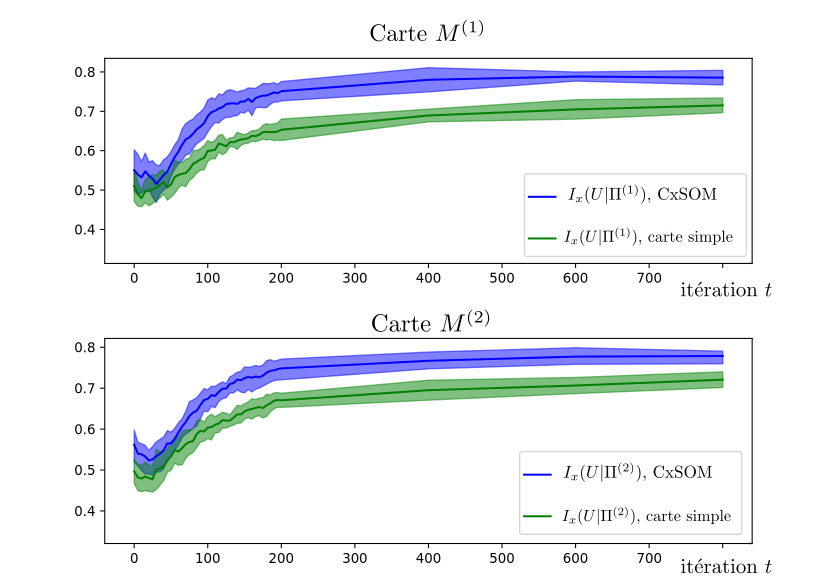
\includegraphics[width=\textwidth]{evolution_MI_binning}
\caption{Evolution de l'information mutuelle normalisée $I_x(U|\bmu)$ dans chaque carte au long de l'apprentissage. La courbe bleue correspond à $I_x(U|\bmu)$ dans l'architecture de cartes $M\m{1}$ et $M\m{2}$. On compare cette évolution à l'évolution de l'information d'une seule carte apprenant sur les mêmes entrées $X$ ou $Y$, sans être connectée.}
\label{fig:MI_evol}
\end{figure}

\subsection{Comparaison des deux méthodes d'estimation}

% Nous avons proposé $I_x$ comme indicateur pour évaluer la relation fonctionnelle entre $U$ et $\bmu$ et noté qu'il est nécessaire de l'estimer par histogrammes pour l'interpréter de cette façon.
% Nous sortons de l'étape de validation de l'indicateur pour comparer deux indicateurs: $I_x$ estimé par histogrammes, et $I_x$ estimé par KNN de Kraskov. Dans cette partie, on considère ces deux valeurs comme deux indicateurs différents. L'estimation par Kraskov est considérée comme l'information théorique, et celle par histogrammes comme l'indicateur représentant la relation fonctionnelle.

% En figure~\ref{fig:MI_evol_total}, nous tracons l'évolution de l'information mutuelle moyenne, cette fois estimée par la méthode de Kraskov. Sur le même schéma, nous tracons également l'évolution de l'information mutuelle obtenue par la méthode des histogrammes. 

% Sur les tracés, l'indicateur calculé avec la méthode de Kraskov converge vers une même valeur à la fin de l'apprentissage pour la carte simple que pour la carte au sein d'une architecture CxSOM (tracés rouges et noirs). Ce résultat est étonnant: cela signifie donc que la carte au sein de CxSOM n'a pas plus d'information sur le modèle que la carte isolée, lorsque cette information est estimée avec la méthode de Kraskov. Ce résultat va également à l'encontre de ce qu'on observe sur l'évolution de l'information mutuelle calculée par les histogrammes, dans laquelle une différence franche est observée entre la carte isolée et la carte au sein de l'architecture.

% Proposons une explication.
% On observe que l'information $I_x(U|\bmu)$ tend vers une même valeur dans CxSOM et dans une carte isolée quand on la calcule avec l'estimateur de Kraskov, plus proche de la valeur théorique de l'information mutuelle. Cela signifie, qu'on a la même quantité d'information sur $U$ avec le BMU, dans la carte isolée que dans CxSOM. Simplement, cette information n'est pas répartie de la même façon. 
% Dans une carte isolée, le niveau de quantification vectorielle qu'on effectue sur $X$ est très précis: lorsqu'on présente une entrée $X$ à la carte, le poids du BMU est très proche de cette valeur $X$ Dans CxSOM, on perd ce niveau de quantification, ce qu'on a observé en figure~\ref{fig:erreur}. Le fait que l'indicateur, lorsqu'il est estimé avec une méthode très granulaire, prend la même valeur dans les deux expériences traduit alors qu'on a perdu de l'information sur l'entrée $X$ par rapport à la carte isolée, avec la perte de précision, mais qu'on a gagné de l'information sur l'autre entrée $Y$. Le fait que les deux évolutions de $I_x$, pour chaque expérience, convergent vers la même valeur montre qu'on est dans une situation de compromis: on gagne de l'information sur le modèle au détriment de l'information sur l'entrée externe.

% C'est donc le fait de discrétiser grossièrement la distribution de $U$ qui permet de mesurer le gain d'information sur le modèle complet, sans prendre en compte le fait que la précision sur l'entrée externe est affaiblie. 
% La comparaison de l'information mutuelle, estimée par Kraskov, entre la carte simple et la carte dans CxSOM nous indique que la quantité d'information totale gagnée par une carte reste identique; elle est simplement répartie différemment entre les deux expériences.

% \begin{figure}
% 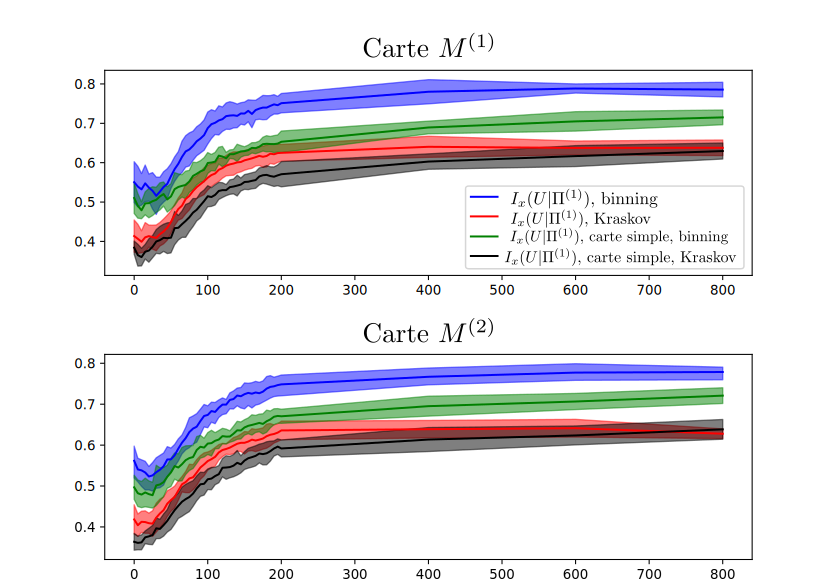
\includegraphics[width=\textwidth]{evolution_MI}
% \caption{Evolution de $I_x(U|\bmu)$ dans chaque carte au long de l'apprentissage, en comparant l'estimation par histogrammes et l'estimation par la méthode de Kraskov.}
% \label{fig:MI_evol_total}
% \end{figure}


\section{Conclusion}
L'indicateur $I_x$ permet donc bien de mesurer s'il existe une relation fonctionnelle entre $U$ et la positio du BMU d'une carte. Cependant, son estimation doit nécessairement être réalisée par histogrammes, avec une grande taille de découpage pour $U$. Ce découpage occulte le fait qu'une position de BMU code pour une zone de valeur de $U$ plus grande que pour une carte classique. 

L'estimation du même indicateur par une méthode plus granulaire et précise nous informe sur le comportement d'une carte.

L'indicateur que nous proposons, $I_x(Y|X) = \frac{I(X,Y)}{H(Y)}$ traduit bien le fait que les cartes ont appris une relation entre les entrées. Son estimation doit passer par une discrétisation avec des intervalles larges pour $U$, afin de ne pas prendre en compte la perte d'information sur l'entrée externe $X$.
Les données doivent égalemement être débruitées avant l'estimation.
Cet indicateur permet de comparer les expériences entre elles.
L'information mutuelle et l'entropie étant des quantités fondamentales en théorie de l'information, il existe de nombreuses méthodes d'estimations de ces valeurs malgré la difficulté qu'elle pose, voir~\cite{Doquire2012ACO} pour une revue de différentes méthodes. Ainsi, de l'information mutuelle normalisée comme indicateur reste robuste pour des données de plus grande dimension ou pour plus de cartes, en utilisant des méthode d'estimations plus élaborées. Cependant, cette estimation devra être retravaillée en plus grande dimension. 

